\documentclass[useAMS, usenatbib]{aastex}
\usepackage{cite,natbib}
\usepackage{epsfig}
\usepackage{cases}
\usepackage[section]{placeins}
\usepackage{graphicx, subfigure}
\usepackage{color}

\title{Systematics-insensitive periodic signal search with K2}

\begin{document}

\date{Draft version 2015 24th of February}
\maketitle

% Aims
From pulsating stars to transiting exoplanets, the search for periodic signals
in {\it K2} data is relevent to a long list of scientific goals.
Systematics affecting {\it K2} light curves due to the decreased
space craft pointing precision inhibit the easy extraction of periodic signals
from the data.
We develop a method for producing periodograms of K2 light curves that
are insensitive to pointing-induced systematics.
% Methods
Sine-fitting periodograms use a generative model to find the frequency
of the sine wave that best describes the data.
We extend this principle by including systematic trends in our generative
model as well as a sum of sine and cosine functions over a grid of
frequencies.
% Results
Using this method we are able to produce periodograms, free from
systematic features.
The quality of the resulting periodograms are such that we can recover acoustic oscillations in giants and detect variable stars, eclipsing binaries and exoplanet
candidates without the need for any detrending.
% Whilst this method performs extremely well in the high part of frequency space,
% relevent for giant asteroseismology, it is not optimised for measuring stellar
% rotation periods.
This method performs well for signals with periods from 1 hour up to 2 days,
however it is not optimized for periods much greater than 5 days.
This is due to the fact that some common trends between stars vary on
timescales similar to rotation periods.

\section{Introduction}
\label{Introduction}

With the failure of {\it Kepler}'s third reaction wheel in 2012, the space
craft was repurposed, and the {\it K2} mission began in 2014.
The excellent precision achieved by the original {\it Kepler} mission relied
on extremely precise pointing, for which three reaction wheels were crucial.
With just two reaction wheels it is still possible to maintain relatively
precise pointing by using the Solar wind to stabilise the space craft and only
observing ecliptic fields.
In this configuration the spacecraft is able to maintain an unstable
equilibrium, with the two reaction wheels controlling pitch and yaw whilst the
spacecraft slowly rolls about the boresight.
The spacecraft fires its thrusters once every $\sim$ 6 hours to correct for
this slow drift.
As stars move across pixels with different sensitivities, their flux varies.
Developing methods for the extraction of information from K2 light
curves, despite the reduced pointing precision, is therefore extremely
important.
Several methods for detrending {\it K2} light curves have already been
developed: \citet{Vanderburg2014} and \citet{Crossfield2015} use simple
aperture photometry and correct the light curve of each star individually.
\citet{Aigrain2015} use a Gaussian process to model the non-linear dependence
of stellar flux on the roll angle of the telescope.
Whilst these methods are successful at removing most of the systematic trends
and produce light curves suitable for exoplanet studies, any signal still
remaining due to the 6 hour thruster fires is detremental to asteroseismic
studies.
A detrending method for {\it K2} light curves, specifically intended for the
asteroseismic analysis of giant stars is being developed by Lund {\it et al.}
(in prep.).
The systematics due to roll are corrected, again on a star-by-star basis and
any remaining periodic signals at 47 $\mu$Hz (6 hour period) or its harmonics
are removed by prewhitening.
We argue that the method developed here, the Systematics-Insenstive
Periodogram (SIP), which produces a periodogram of the data without the need
for detrending is prefereable for asteroseismic studies.

The {\it Kepler} spacecraft is currently observing its 4th field and data for
campaigns 0 and 1 have been released.
Within these fields there are thousands of variable stars, rotating stars,
pulsating stars and exoplanet hosts.
The original {\it Kepler} mission provided a huge set of light curves with
periodic behaviour on timescales ranging from a few minutes to a few months.
The field of asteroseismology, to name just one, was enormously advanced by
its excellent precision.
Fundamental stellar parameters---in some cases, extremely precise ones---can
be calculated for {\it Kepler} asteroseismic stars from the power spectra of
their light curves.
% Around 600 Solar-like oscillators, pulsating at $\sim$5 minute to
% $\sim$hour-long timescales, were observed in short cadence mode.
The asteroseismic pulsations of giant stars lie below the Nyquist frequency set
by the 28.5 minute sampling rate of long cadence {\it Kepler} data:
283 $\mu$Hz.
% The Fast Fourier Transform (FFT) and sine-fitting periodogram are fundamental
% tools in the asteroseismic toolbox.
Asteroseismic analysis of {\it Kepler} data is traditionally conducted upon
detrended light curves.
For short cadence {\it Kepler} data, this detrending method is described in
\citet{Garcia2011}.

Stellar rotation periods can be extracted from {\it Kepler} light curves;
active regions on the surface of rotating stars produce periodic variations
in flux.
Stellar rotation is a field of active interest as the rotation period of star
can be used to infer its age \citep{Skumanich1972, Barnes2007, Epstein2014},
is thought to be tied to the magnetic dynamo, and could even reveal dynamical
interations with companion stars or planets
\citep[e.g.][]{Beky2014, Poppenhaeger2014}.
% Rotation periods are also useful for {\it Kepler} exoplanet characterization.
% Active regions can produce variability in radial velocity as well as
% photometry and can masquerade as planetary signals.
% It is therefore extremely useful to be able measure the rotation period of the
% star directly from the light curve.
Current methods for measuring rotation periods from {\it Kepler} light curves
include periodogram \citep[e.g.][]{Reinhold2013}, AutoCorrelation Function
(ACF) \citep{McQuillan2013} and wavelet \citep[e.g.][]{Garcia2014} analysis,
or some combination thereof.
Stellar variability is not typically sinusoidal, therefore sine-fitting
periodograms are not perfectly suited for measuring rotation periods.
For this reason, the ACF method is often favoured over the periodogram method.
However, because autocorrelation is performed on the data, not a generative
model, we cannot use autocorrelation techniques on non-detrended {\it K2} data.
A quasi-periodic Gaussian process is a much better effective model for stellar
variability, however we are not only concerned with stellar rotation and choose
to focus on the more generally applicable (and computationally tractable)
sine-wave periodogram, leaving the Gaussian process for future work.

Aside from asteroseismology and stellar rotation there are many other fields
of research, targeted by {\it K2} that utilize periodic information.
These include searching for eclipsing binaries, variable stars and exoplanets,
and even studying white dwarfs and AGN.
The development of tools for extracting periodic information from {\it K2}
data is essential if it is to be as revolutionary in time-domain
astronomy as its former incarnation was.

\section{Method}
\label{Method}

The method implemented in this paper is an extention of the planet-search
algorithm developed by \citet{Foreman-Mackey2015} (hereafter FM15).
All targets observed by {\it Kepler} move on the CCD in the same way and
therefore the systematics affecting each individual star's light curve have
shared properties.
The FM12 method utilizes the fact that pointing-induced systematics are shared
across stars and decomposes the trends into a set of `Eigen Light Curves'
(ELCs) using Principle Component Analysis (PCA).
This method is similar to that used to produce PDC-MAP data for the original
{\it Kepler} mission \citep[][]{Stumpe2012, Smith2012}.
The resulting ELCs can then be used to model any campaign 1 {\it }light
curve with an arbitrary physical model.
FM15 downloaded the target pixel files for all stars observed in campaign 1;
21,703 in total.
The position of each star was predicted using the world coordinate system and
10 circular apertures placed around the star with radii varying from 1 to
5 pixels in steps of 0.5 pixels.
Following the procedure of \citet{Vanderburg2014}, the aperture producing the
light curve with the lowest CDPP with a 6 hour window \citet{Christiansen2012}
was selected.
PCA was then performed on the full set of targets in order to produce ELCs.
FM15 used 150 of these ELCs with a transit model in order to
search for exoplanet candidates without the need for a `detrending' step.
The likelihood of the data, conditioned on their ELC-plus-transit
model was calculated over a fine grid of periods and transit depths, resulting
in the detection of 36 new exoplanet candidates.
We use exactly the same technique to find periodic signals in {\it K2} data,
however, instead of a transit model, we use a sum of sine and cosine functions.
The model is linear, therefore the likelihood function conditioned on
a specific frequency can be calculated and the systematics model marginalized
over analytically.

Following the notation in FM15, our model for the $k$th star can be written
\begin{equation}
	\mathbf{f_k} = \mathbf{A}\mathbf{w_k} + \mathrm{noise},
\end{equation}
where $\mathbf{f_k}$ is the vector of $N$ flux values,
\begin{equation}
	\mathbf{f_k} = (f_{k,1}, f_{k,2}, f_{k,3}, ..., f_{k,N})^T
\end{equation}
at times
\begin{equation}
	\mathbf{t_k} = (t_1, t_2, t_3, ..., t_N)^T.
\end{equation}
$\mathbf{A}$ is the design matrix:
\begin{eqnarray}
	\mathbf{A} &=& \left (\begin{array}{ccccccc}
	x_{1,1} & x_{2,1} & \cdots & x_{150,1} & 1 & \sin(2\pi\nu t_1) & \cos(2\pi\nu t_1) \\
	x_{1,2} & x_{2,2} & \cdots & x_{150,2} & 1 & \sin(2\pi\nu t_2) & \cos(2\pi\nu t_2\\
    && \vdots &&&\\
	x_{1,N} & x_{2,N} & \cdots & x_{150,N} & 1 & \sin(2\pi\nu t_N) & \cos(2\pi\nu t_N)
\end{array}\right )
\end{eqnarray}
where the $x_{ij}$s are the ELCs, with $i$ denoting the ELC number and $j$ the
time index. The maximum likelihood solution for the weight vector,
$\mathbf{w}$ is
\begin{equation}
	\mathbf{w_k}^* \gets (\mathbf{A}^T\mathbf{A})^{-1}\mathbf{A}^T\mathbf{f_k} \end{equation}

\section{Application to asteroseismology}

An example Lomb-Scargle periodogram\footnote{All Lomb-Scargle periodograms
produced in this project were calculated using the gatspy Python module:
https://github.com/astroML/gatspy/tree/master/gatspy/periodic}
of the raw {\it K2 photometry} for EPIC 201211472 is shown in figure
\ref{fig:raw}.
Peaks appearing at 47 $\mu$Hz and its harmonics are produced by the regular
$\sim$ 6 hour thruster fires that repoint the spacecraft.
These peaks are also present in periodograms of the \citet{Vanderburg2014}
detrended light curves.
The presence of systematic signals at these timescales are problematic for
asteroseismic analysis since they lie in the region of frequency space
populated by giant asteroseismic modes.
It is possible to remove these signals by `prewhitening' the data, i.e.
removing a sine wave at that frequency from the data, however no such
procedure is necessary for our method.

We selected long cadence targets from the GO1059 proposal: "Galactic
Archaeology on a grand scale" (PI: Stello, D.) in order to test our method.
Periodograms of the raw data were produced by calculating the signal to noise
ratio of the amplitudes of single sine and cosine functions and 150 ELCs
conditioned on the data at a range of frequencies.
In order to identify acoustic modes we searched for a power excess in these
periodograms using the method described in \citet{Huber2009}.
Autocorrelation functions are calculated for sections of the power spectrum in
order to search for regions of increased correlation.
The increased correlation arises from the even frequency spacing of acoustic
modes, and the frequency of maximum correlation at the location of the power
excess corresponds to the large frequecy separation, $\Delta\nu$.
Figures \ref{fig:1} to \ref{fig:6} show example power spectra of 6 targets for
which we detect pulsations using this method.

% Our method does not perfectly model the systematics for every star.
% Of the power spectra generated for each of the n stars in GO1049, n of them
% showed power at 47$\mu$Hz.
% Examples of power spectra containing residual systematic features are shown in
% figure ?.

We applied our analysis to 3 red giants and 3 $\delta$ Scuti stars
identified by Lund {\it et al.} (in prep), in campaign 0.
Since campaign 0 was shorter, $\sim$ 25 days, our method is not as successful
at modelling the systematics as for campaign 1.
% and fewer stars observed?
For this reason the 47$\mu$Hz peaks caused by the regular 6 hour thruster
firings appear, with relatively high amplitudes for 2 of the 6 targets and with
moderate amplitudes for another 2 of the 6.
Two of the most sucessful periodograms, for targets EPIC 202086286 and EPIC
202068435 are shown in figure \ref{fig:c0}.

\section{Application to stellar rotation}
The top panel of figure \ref{fig:rotation_poster_child} shows the light curve
of an active, rotating star, EP201317002.
This light curve has been detrended using the method of
\citet{Vanderburg2014}.
The middle and bottom panels show an ACF and Lomb-Scargle periodogram of the
detrended light curve.
The highest peaks in both the ACF and periodogram are located at around 10
days.
Figure \ref{fig:K2_rotation_poster_child} shows the raw light curve of the same
target with a periodogram calculated by modeling the data as a linear
combination of ELCs and a sine and cosine function at a range of
frequencies.
Each method measures a rotation period of around 10 days for this target.

Figure \ref{fig:top5} shows the 5 ELCs with the highest weights
for this star.
Most of these ELCs vary on timescales close to 10 days.
The light curve of EPIC 201317002 is therefore easily described by the ELCs
alone, without the need for an additional sinusoidal signal.

\section{Injections with sinusoids}

In order to test the sensitivity, completeness and reliability of this method
we injected sinusoids into real {\it K2} light curves.

EPIC 201311941 was identified as a quiet star with no significant periodic
variability at any frequency.
1000 sinusoids with periods ranging (linearly in log-space) from 1 to 50 days
and varying amplitudes were injected into the raw light curve of EPIC
201311941.
The amplitudes ranged from 1 to 1000 parts-per-million, again linearly in
log-space.
20 different amplitudes were tested, so 20,000 injections were performed in
total.
The highest peak in the resulting periodogram of each light curve was recorded.
If the period of the highest peak lay within 10\% of the true period, it was
considered a successful detection.
This procedure was repeated for periods ranging from 1 hour to 2 days in order
test the recovery of signals at frequencies relevent to asteroseismology.
The resulting completeness maps are shown in figures \ref{fig:K2_hist_r} and
\ref{fig:K2_hist_a}.

\section{Discussion}

\subsection{Further examples}
Figure \ref{fig:RRLyrae} shows the periodogram of an RR Lyrae star, selected
from Guest observing program GO1018 and figure
\ref{fig:EB} shows the periodogram of an EB, selected from
\citet{Armstrong2015}.
Figure \ref{fig:planet} shows the same thing for a short-period planet
candidate.
This planet has a period of around 0.4 days, short enough to be detectable
with a periodogram, as was demonstrated for a number of ultra-short
period {\it Kepler} exoplanets by \citet{Sanchis-Ojeda2014}.
The top panels of these three figures show the {\it K2} light curves of these
objects, conditioned on the highest amplitude sinusoidal signal in the
periodograms.

Photometric variability in dwarf stars on timescales less than 8 hours, often
known as flicker, has been linked with surface gravity, g
\citep[][]{Bastien2013, Kipping2014}.
The metrics used to quantify photometric variability include finding the range
in intensity, counting the number of zero crossings and calculating the
root-mean-square (RMS) of the light curve.
Although related to periodic analysis these are all operations performed on the
a detrended light curve, they are not inferred from a periodogram.
However, it may be possible to derive a property of the periodogram that scales
with the density or surface gravity of a star, for example, the mean excess
power at frequencies near those relevent to granulation timescales.

\section{Conclusions}
We have demonstrated that modelling {\it K2} photometry as a linear combination
of 150 PCA components plus a sinusoid can produce beautiful periodograms
without the need for detrending.
We find that the 47 $\mu$Hz signal, generated by the space craft thruster
fires is not present in the vast majority of SIPs for more than 4000 targets
selected from the {\it K2} guest observer program, GO1059, "Galactic
Archaeology on a grand scale" (PI: Stello, D.).
The SIP method is highly successful for campaign 1 targets where the large
number of stars, observed for a baseline of 80 days ensures that most of the
systematics are captured in the ELCs and we anticipate that is will
be equally effective for the up-and-coming campaigns.

The successes of the SIP method are most apparent in the high frequency regime,
particularly in the region of frequency space relevent to the study of
asteroseismic oscillations in giant stars.
SIP also performs well for signals with periods between $\sim$ 1 hour and
$\sim$ 2 days, however it is not well optimised for measuring stellar rotation
periods, due to the fact that many ELCs are dominated by periodic variations
on the same timescales as the rotation periods.

\begin{figure*}
\begin{center}
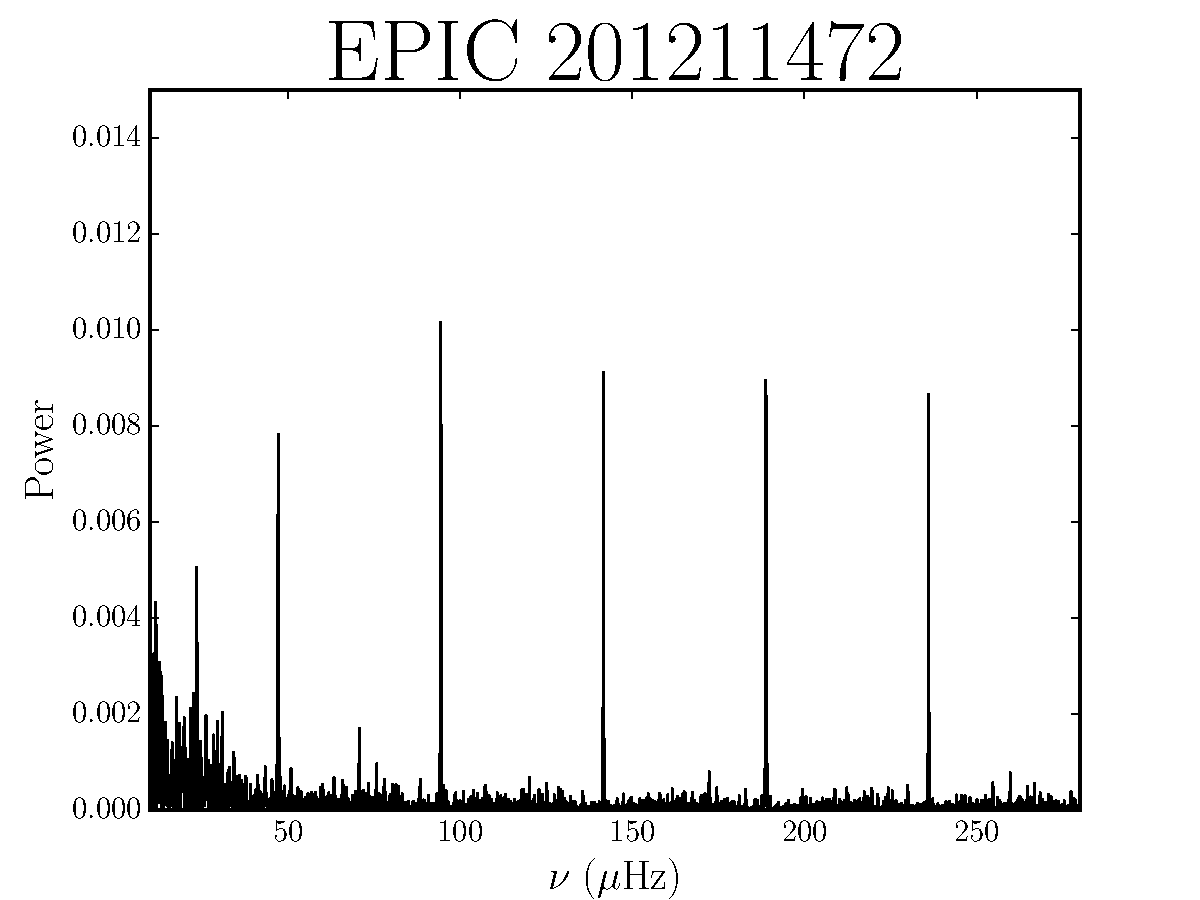
\includegraphics[width=6in, clip=true]{raw_201211472.pdf}
\caption{Lomb-scargle periodogram of the raw {\it K2} photometry for
	EPIC 201211472.}
\label{fig:raw}
\end{center}
\end{figure*}

\begin{figure}
\begin{center}
	\subfigure[]{
            \label{fig:1}
	    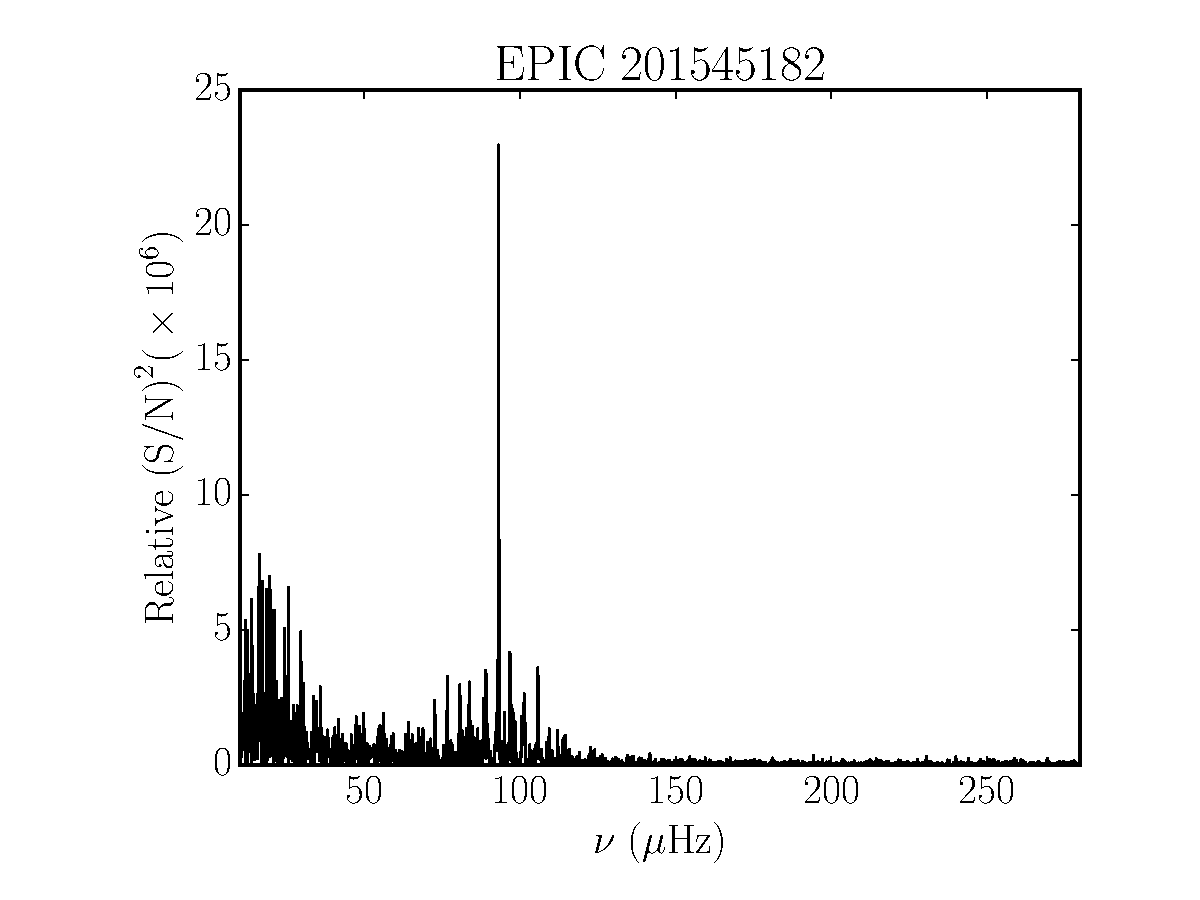
\includegraphics[width=3in]{201545182.pdf}
        }
	\subfigure[]{
            \label{fig:2}
	    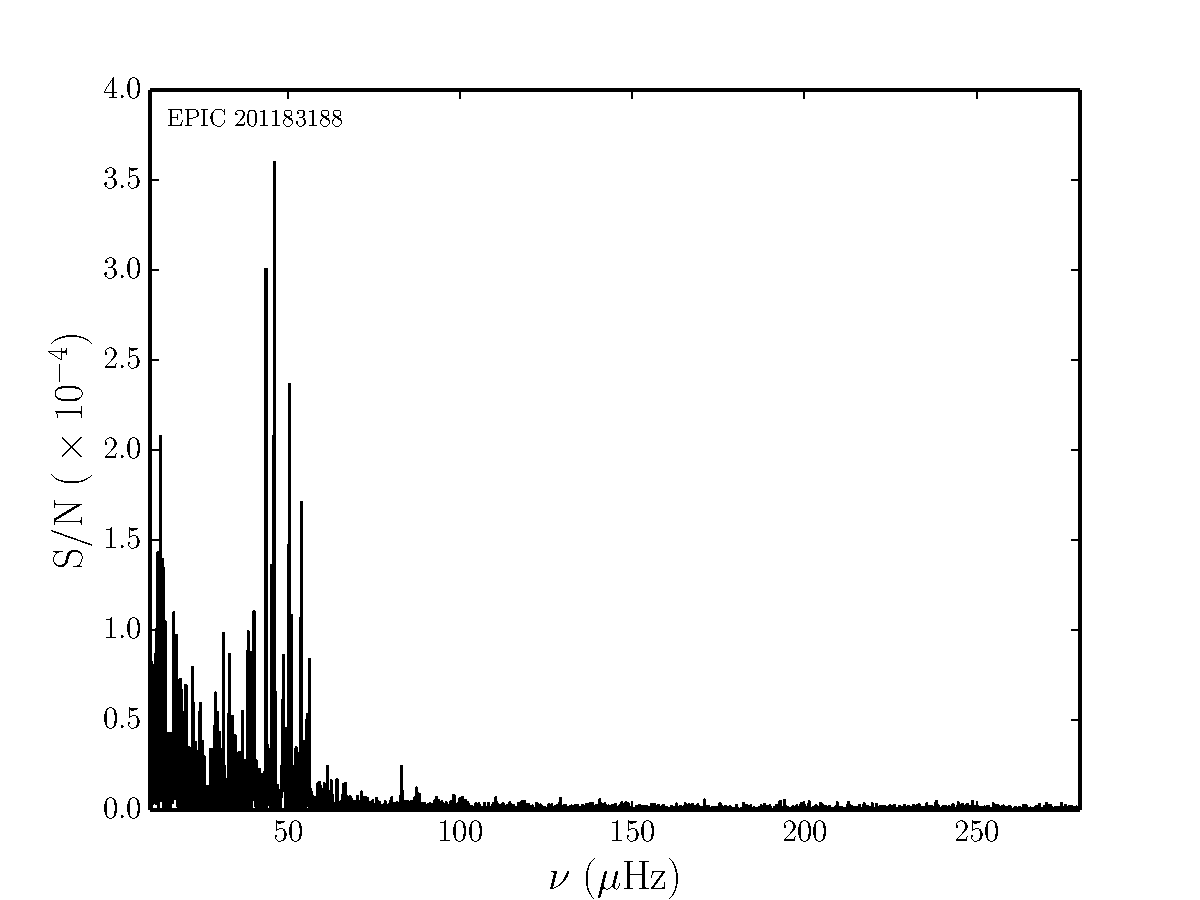
\includegraphics[width=3in]{201183188.pdf}
        }
	\subfigure[]{
            \label{fig:3}
	    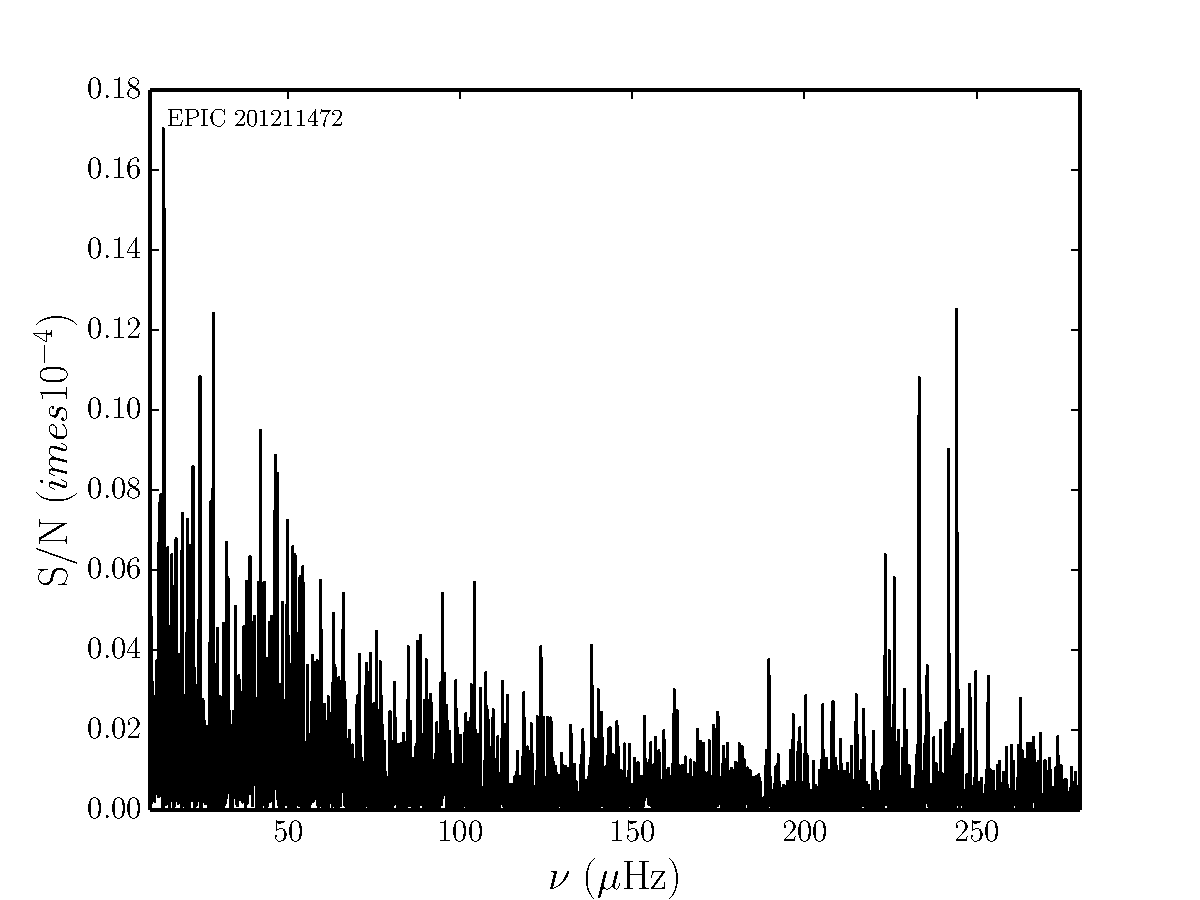
\includegraphics[width=3in]{201211472.pdf}
        }
	\subfigure[]{
            \label{fig:4}
	    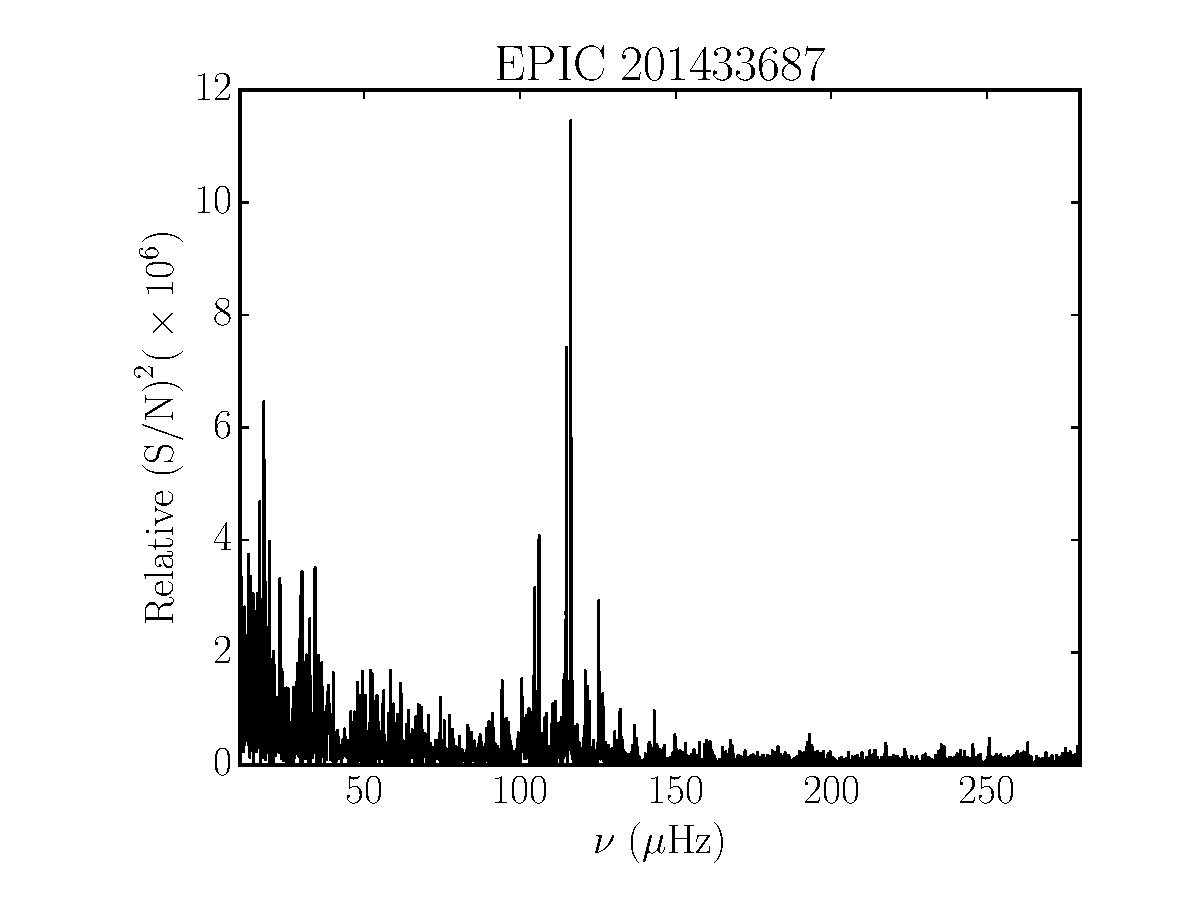
\includegraphics[width=3in]{201433687.pdf}
        }
	\subfigure[]{
            \label{fig:5}
	    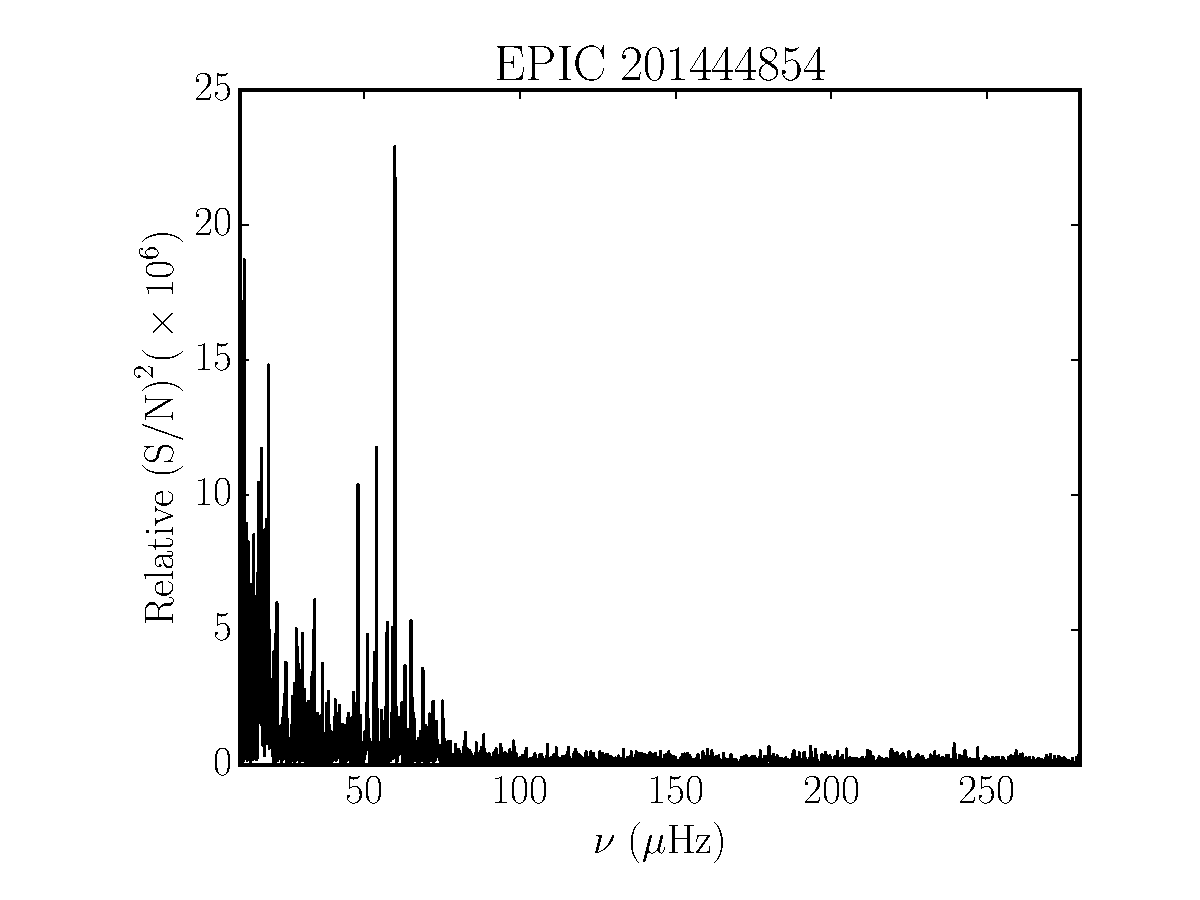
\includegraphics[width=3in]{201444854.pdf}
        }
	\subfigure[]{
            \label{fig:6}
	    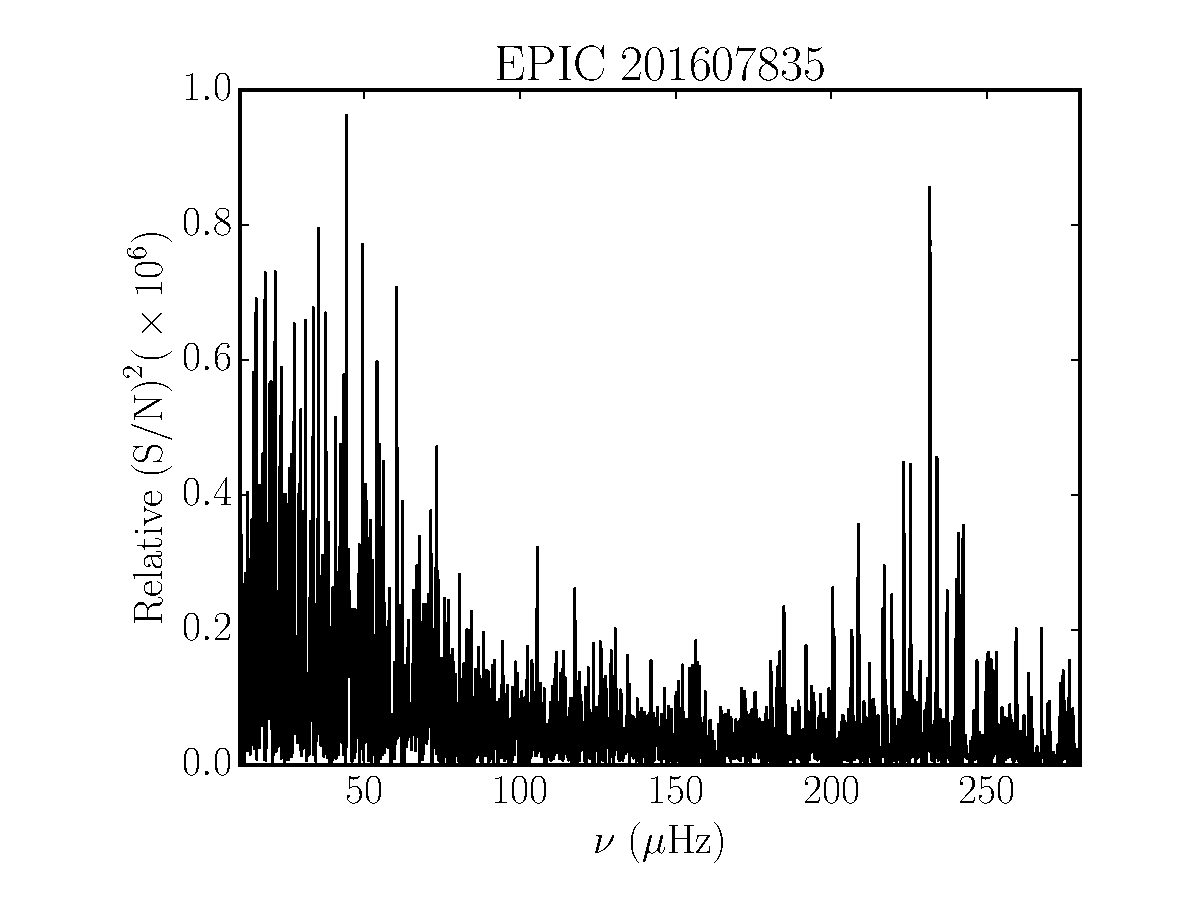
\includegraphics[width=3in]{201607835.pdf}
        }
    \end{center}
    \caption{SIPs of 6 long cadence {\it K2} giants with pulsations.
\label{fig:astero_examples}}
\end{figure}

\begin{figure}
\begin{center}
	\subfigure[]{
            \label{fig:c01}
	    \includegraphics[width=3in]{202086286.pdf}
        }
	\subfigure[]{
            \label{fig:c02}
	    \includegraphics[width=3in]{202068435.pdf}
        }
    \end{center}
    \caption{SIPs of 2 long cadence {\it K2} giants with
	    pulsations from campaign 0. These targets were identified as
	    pulsating giants by Lund {\it et al.} (in prep).
\label{fig:c0}}
\end{figure}

\begin{figure*}
\begin{center}
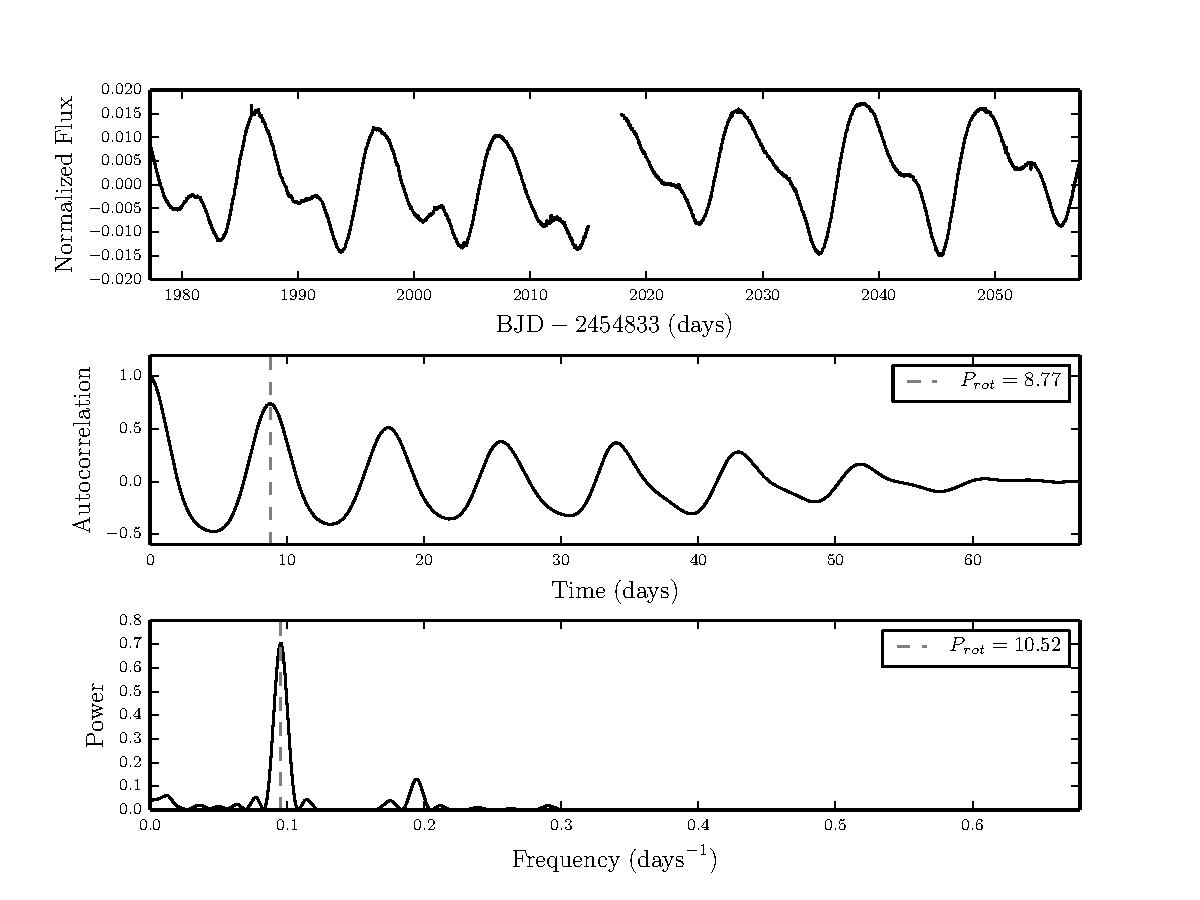
\includegraphics[width=6in, clip=true]{rotation_poster_child.pdf}
\caption{{\it Top}: Light curve of EP201317002, detrended using the method
of \citet{Vanderburg2014}. {\it Middle}: Autocorrelation function of the
light curve. The autocorrelation function method measures a rotation period of
8.77 days for this star. {\it Bottom}: The Lomb-Scargle periodogram of the
light curve. The highest peak in the periodogram is centred at 10.52 days.}
\label{fig:rotation_poster_child}
\end{center}
\end{figure*}

\begin{figure*}
\begin{center}
\includegraphics[width=6in, clip=true]{K2_rotation_201317002.pdf}
\caption{{\it Top}: Raw light curve of EP201317002. {\it Bottom}: A
periodogram produced by modelling the data using the top 150 ELCs
plus a sine and cosine function at a range of frequencies. The highest peak in
the periodogram is centred at 10.34 days.}
\label{fig:K2_rotation_poster_child}
\end{center}
\end{figure*}

\begin{figure*}
\begin{center}
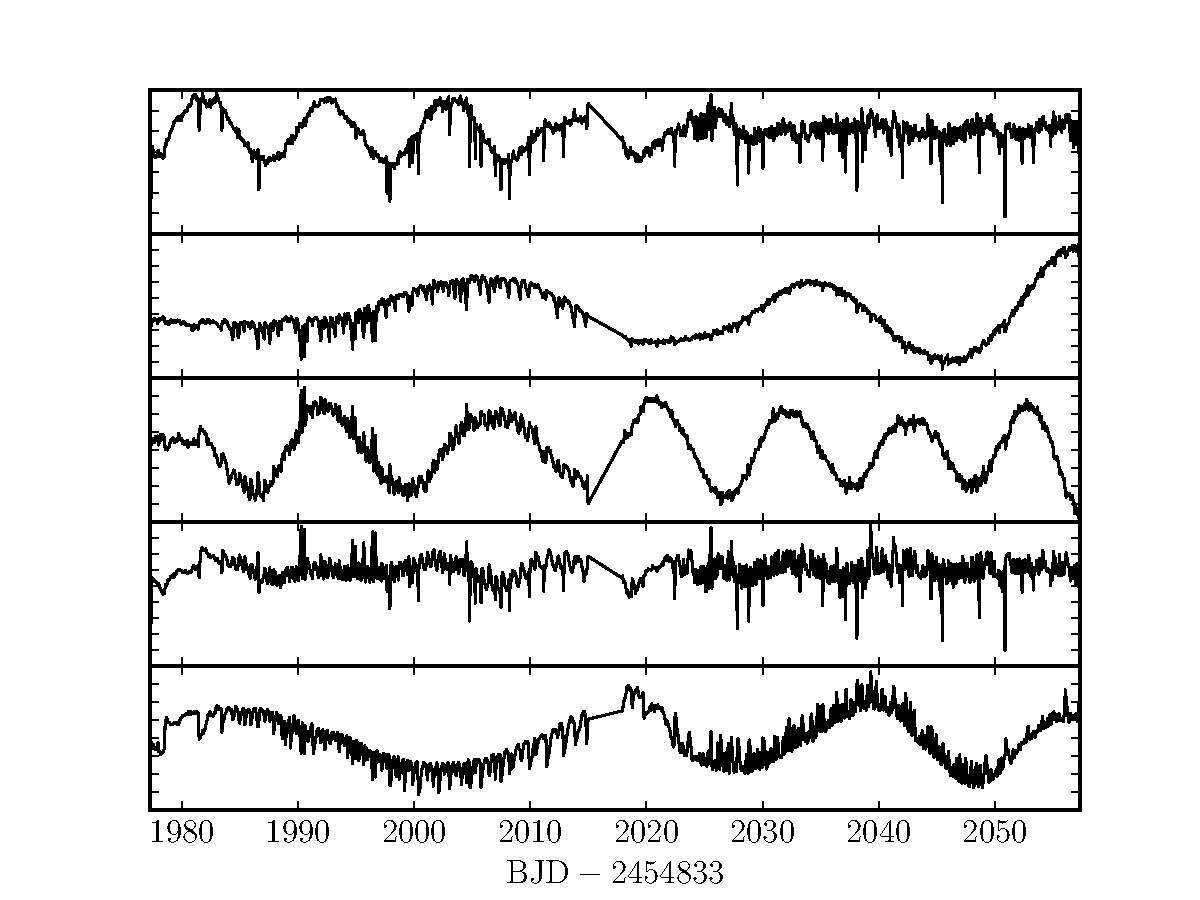
\includegraphics[width=6in, clip=true]{201317002_top5.pdf}
\caption{The 5 highest-weighted ELCs for EPIC 201317002,
illustrating the problem with measuring rotation periods.}
\label{fig:top5}
\end{center}
\end{figure*}

\begin{figure*}
\begin{center}
\includegraphics[width=6in, clip=true]{K2_hist_r.pdf}
\caption{Completeness of sinusoidsal signal recovery. 20,000 Sinusoidal signals
with a range of periods and amplitudes were injected into the raw light curve
of the non-variable star EPIC 201311941. In the range of periods relevent to
stellar rotation ($\sim$ 0.5 - 60 days), we are most complete at the shortest
periods.}
\label{fig:K2_hist_r}
\end{center}
\end{figure*}

\begin{figure*}
\begin{center}
\includegraphics[width=6in, clip=true]{K2_hist_a.pdf}
\caption{Completeness of sinusoidsal signal recovery. 20,000 Sinusoidal signals
with a range of periods and amplitudes were injected into the raw light curve
of the non-variable star EPIC 201311941. In the range of periods relevent to
asteroseismology ($\sim$ 1 - 48 hours), we are uniformily complete down to
very low amplitudes.}
\label{fig:K2_hist_a}
\end{center}
\end{figure*}

\begin{figure*}
\begin{center}
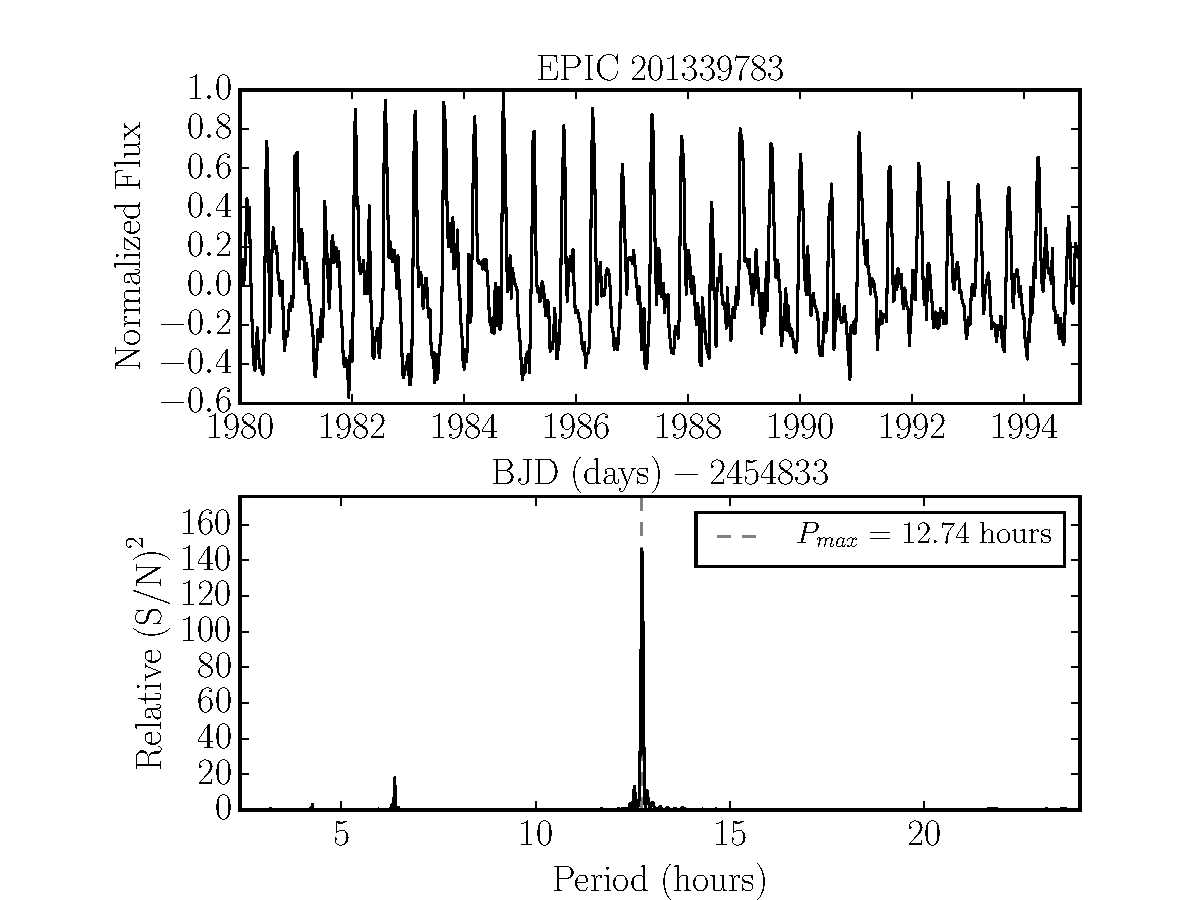
\includegraphics[width=4in, clip=true]{RR_201339783.pdf}
\caption{{\it Top:} The light curve of RR Lyrae star, EPIC 201339783,
	conditioned on the highest amplitude sinusoidal signal found in the
	periodogram. {\it Bottom:} The systematic-insensitive periodogram of
	this target.}
\label{fig:RRLyrae}
\end{center}
\end{figure*}

\begin{figure*}
\begin{center}
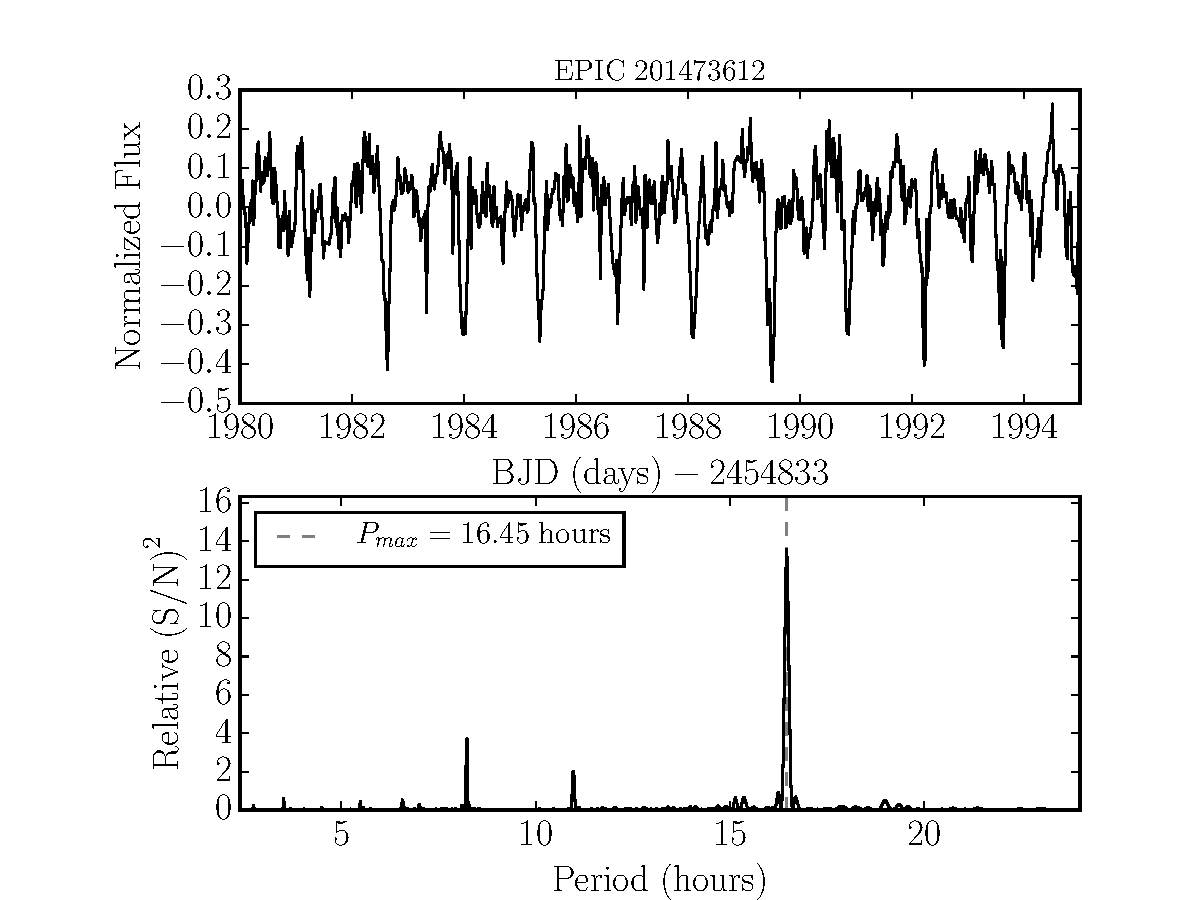
\includegraphics[width=4in, clip=true]{EB_201473612.pdf}
\caption{{\it Top:} The light curve of eclipsing binary, EPIC 201473612,
	conditioned on the highest amplitude sinusoidal signal found in the
	periodogram. {\it Bottom:} The systematic-insensitive periodogram of
	this target.}
\label{fig:EB}
\end{center}
\end{figure*}

\begin{figure*}
\begin{center}
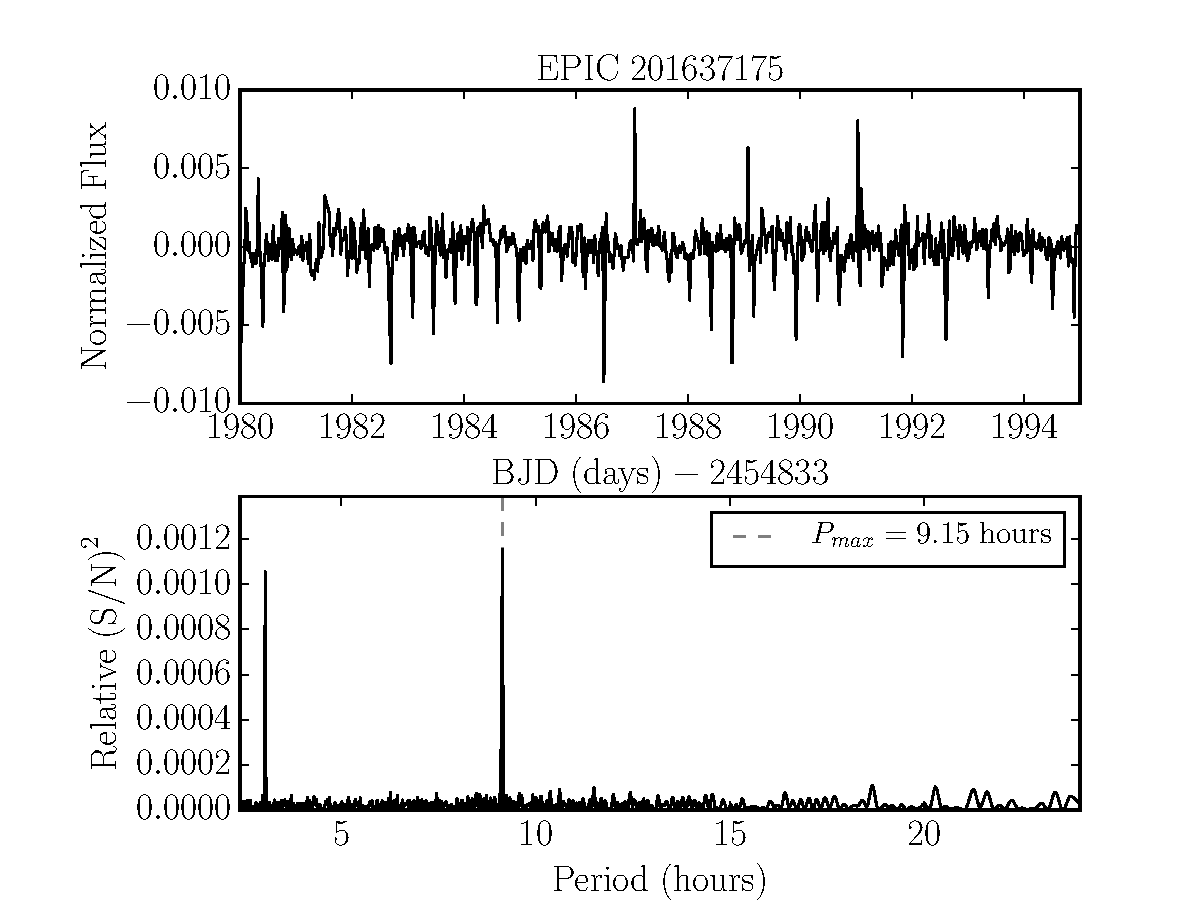
\includegraphics[width=4in, clip=true]{planet_201637175.pdf}
\caption{{\it Top:} The light curve of exoplanet candidate, EPIC 201637175,
	conditioned on the highest amplitude sinusoidal signal found in the
	periodogram. {\it Bottom:} The systematic-insensitive periodogram of
	this target.}
\label{fig:planet}
\end{center}
\end{figure*}

\bibliographystyle{plainnat}
\bibliography{k2rotation}
\end{document}
